% --------------------------------------------------------------
% This is all preamble stuff that you don't have to worry about.
% Head down to where it says "Start here"
% --------------------------------------------------------------
 
\documentclass[12pt]{article}
 
\usepackage[margin=1in]{geometry} \usepackage{amsmath,amsthm,amssymb}
\usepackage{minted}
\usepackage{graphicx}
\graphicspath{ {screenshots/} }


 
\newcommand{\N}{\mathbb{N}}
\newcommand{\Z}{\mathbb{Z}}
 
\newenvironment{theorem}[2][Theorem]{\begin{trivlist}
\item[\hskip \labelsep {\bfseries #1}\hskip \labelsep {\bfseries #2.}]}{\end{trivlist}}
\newenvironment{lemma}[2][Lemma]{\begin{trivlist}
\item[\hskip \labelsep {\bfseries #1}\hskip \labelsep {\bfseries #2.}]}{\end{trivlist}}
\newenvironment{exercise}[2][Exercise]{\begin{trivlist}
\item[\hskip \labelsep {\bfseries #1}\hskip \labelsep {\bfseries #2.}]}{\end{trivlist}}
\newenvironment{problem}[2][Problem]{\begin{trivlist}
\item[\hskip \labelsep {\bfseries #1}\hskip \labelsep {\bfseries #2.}]}{\end{trivlist}}
\newenvironment{question}[2][Question]{\begin{trivlist}
\item[\hskip \labelsep {\bfseries #1}\hskip \labelsep {\bfseries #2.}]}{\end{trivlist}}
\newenvironment{corollary}[2][Corollary]{\begin{trivlist}
\item[\hskip \labelsep {\bfseries #1}\hskip \labelsep {\bfseries #2.}]}{\end{trivlist}}

\newenvironment{solution}{\begin{proof}[Solution]}{\end{proof}}
 
\begin{document}
 
% --------------------------------------------------------------
%                         Start here
% --------------------------------------------------------------
 
\title{Homework 7}
\author{Iman Tabrizian\\ %replace with your name
ECE1508}

\maketitle

\vspace{5mm} 
\textbf{Part 1.1}

\vspace{2mm} 

\vspace{5mm} 

\textbf{4.1}

\vspace{2mm} 

It seems like that during the nights the traffic is much higher than the days. 
Especially, around 10 pm the traffic in most areas is more than the other time during the 24 hours. \\


\vspace{5mm} 

\textbf{4.2}

\vspace{2mm} 

\begin{enumerate}
	\item Graph shows whether the current traffic speed is more than the highway free flow speed or not.
	\item It seems like for some highways during the night the traffic speed is slow. But generally the highways that I have selected have a moderate traffic ratio.
	\item When p is more than 1 this indicates that the speed of cars traversing the highway is more than the number that could freely drive. 
	\item Yes, for most of the highways that I have selected the p ratio is more than 1.

\end{enumerate}

\vspace{5mm} 
\textbf{Part 1.2}

\vspace{2mm} 


The bixi load specifies the ratio of the bikes in use. The load shows when
there are more number of bikes in use. It seems like bike usage during night
is following a steady state and is constant. \\

\vspace{5mm} 
\textbf{Part 2}

\vspace{2mm} 

\vspace{5mm} 
\textbf{2.}

\vspace{2mm} 

There is a pattern in the AQI index. For some cities the pattern is monotonic and suddenly drops (possible as a result of rain or wind). But for some other cities it is always in the same level. Shanghai seems to be more polluted than most of the other cities.

There is a pattern in the Open Weather API data collected over 24 hours. Some of the cities actually have fewer weather fluctuations, where as other cities show more stable weather.


\vspace{5mm} 
\textbf{3.}

\vspace{2mm} 

It seems like cold weather exacerbates the pollution because of the inversion happening. This pattern was concieved in some cities while not in the others.

\begin{figure}[h]
	\centering
	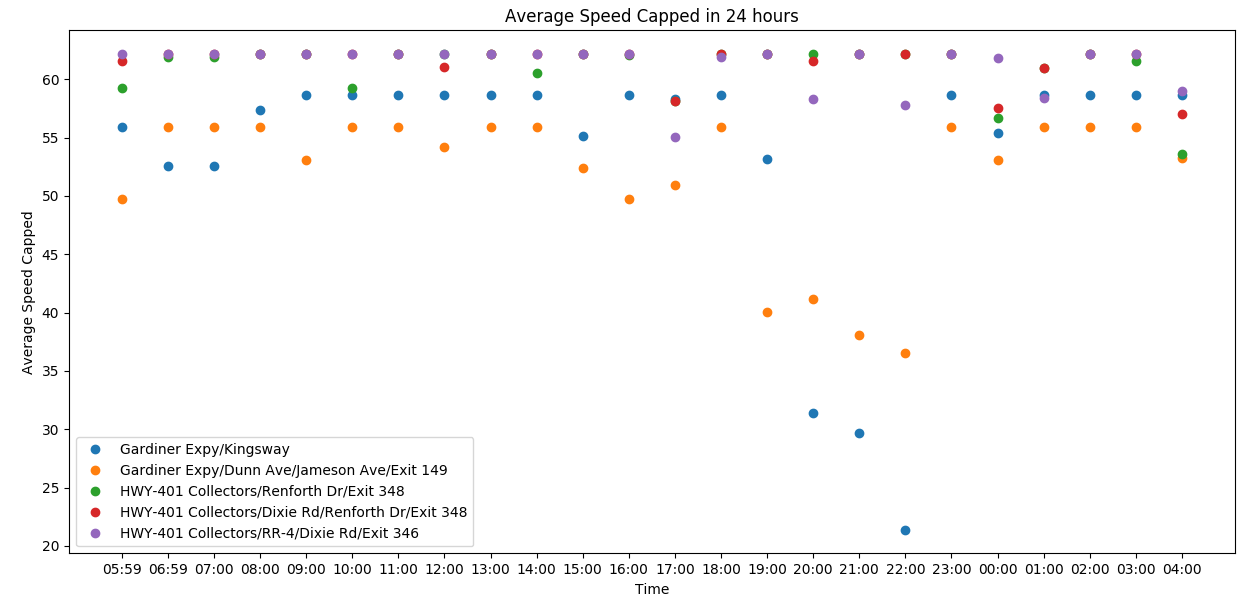
\includegraphics[scale=0.4]{traffic-graph-1}
	\caption{Traffic Graph 1}
\end{figure}

\begin{figure}[h]
	\centering
	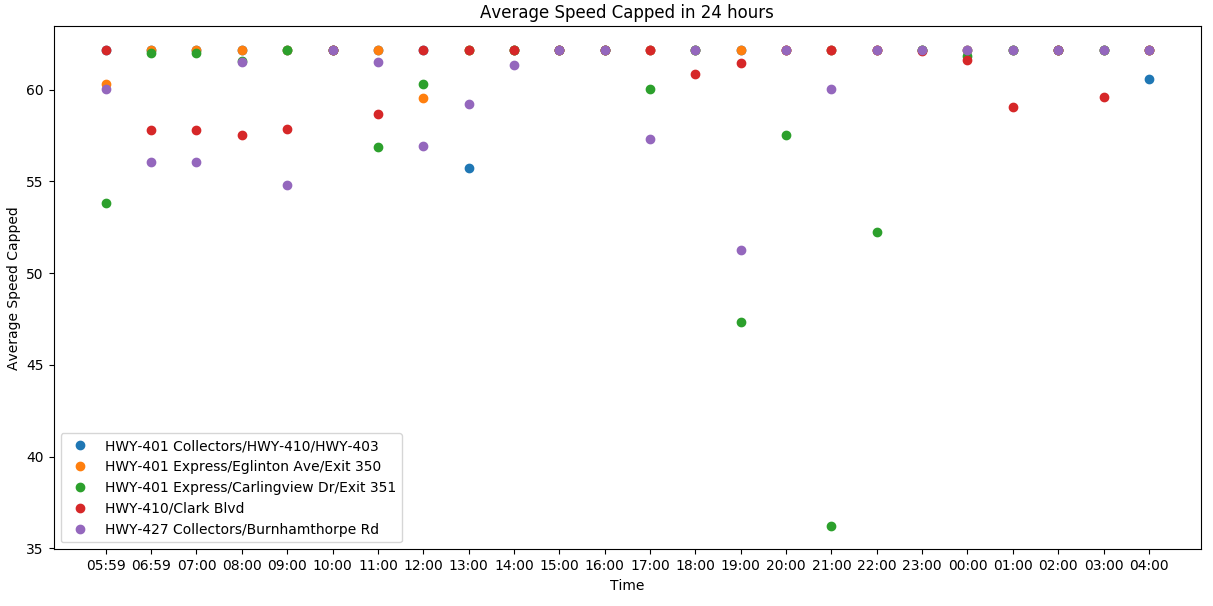
\includegraphics[scale=0.4]{traffic-graph-2}
	\caption{Traffic Graph 2}
\end{figure}

\begin{figure}[h]
	\centering
	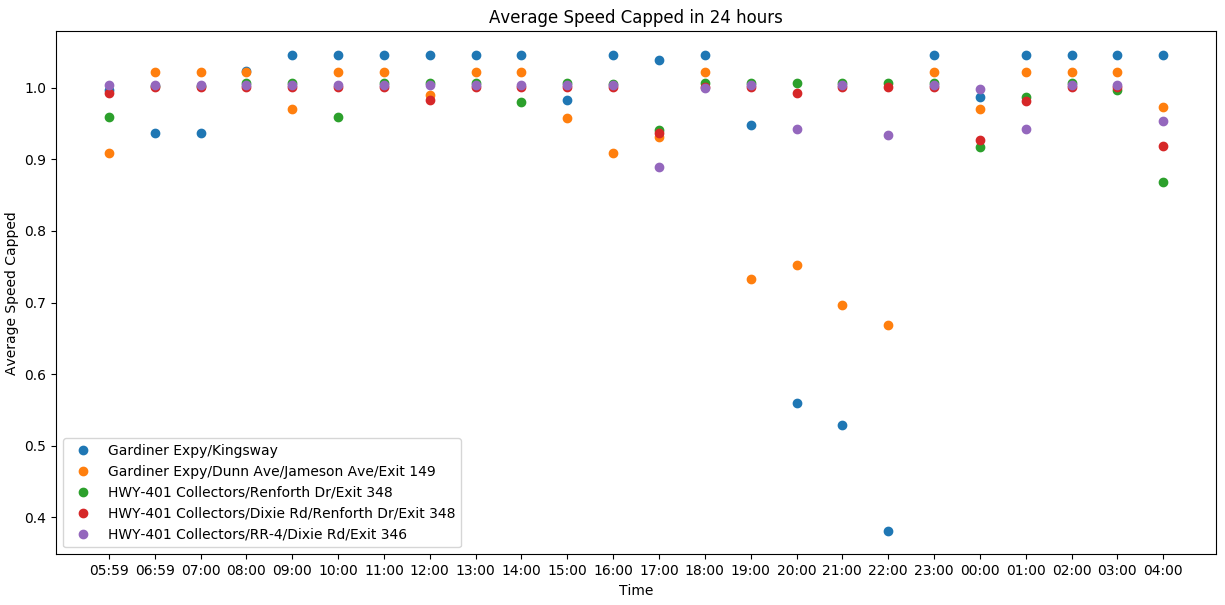
\includegraphics[scale=0.4]{traffic-graph-p-1}
	\caption{Traffic Graph 1 - p index}
\end{figure}

\begin{figure}[h]
	\centering
	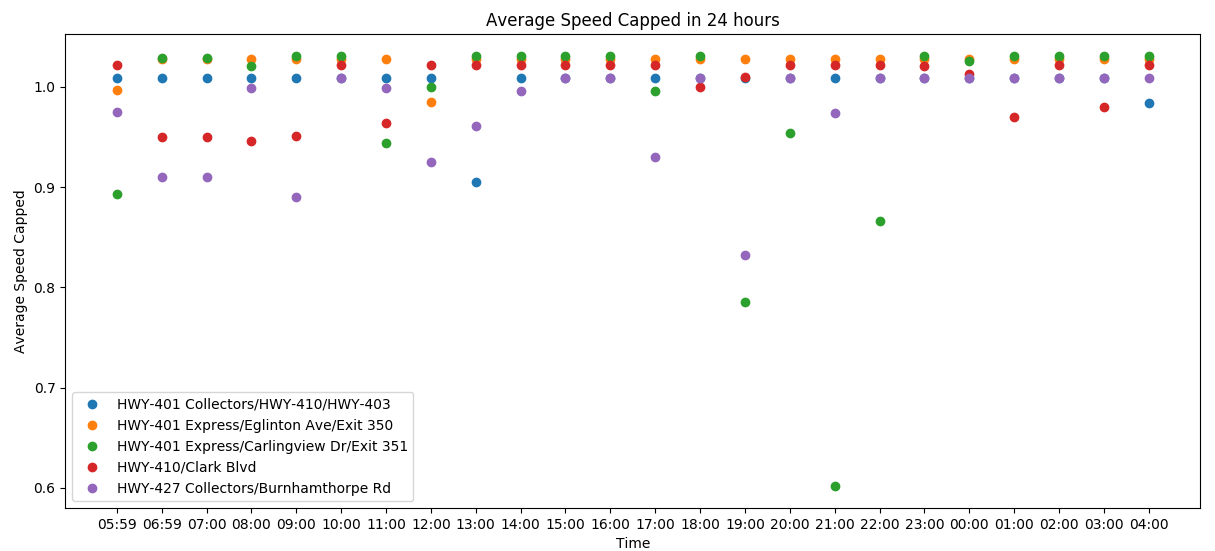
\includegraphics[scale=0.4]{traffic-graph-p-2}
	\caption{Traffic Graph 2 - p index}
\end{figure}

\begin{figure}[h]
	\centering
	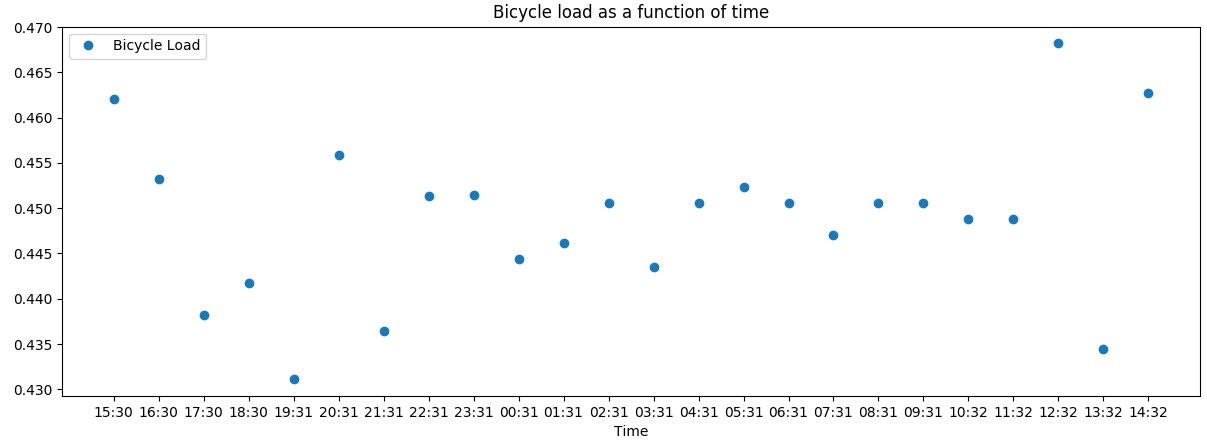
\includegraphics[scale=0.4]{bixi-graph-1}
	\caption{BIXI Bicycles Graph}
\end{figure}


\begin{figure}[h]
	\centering
	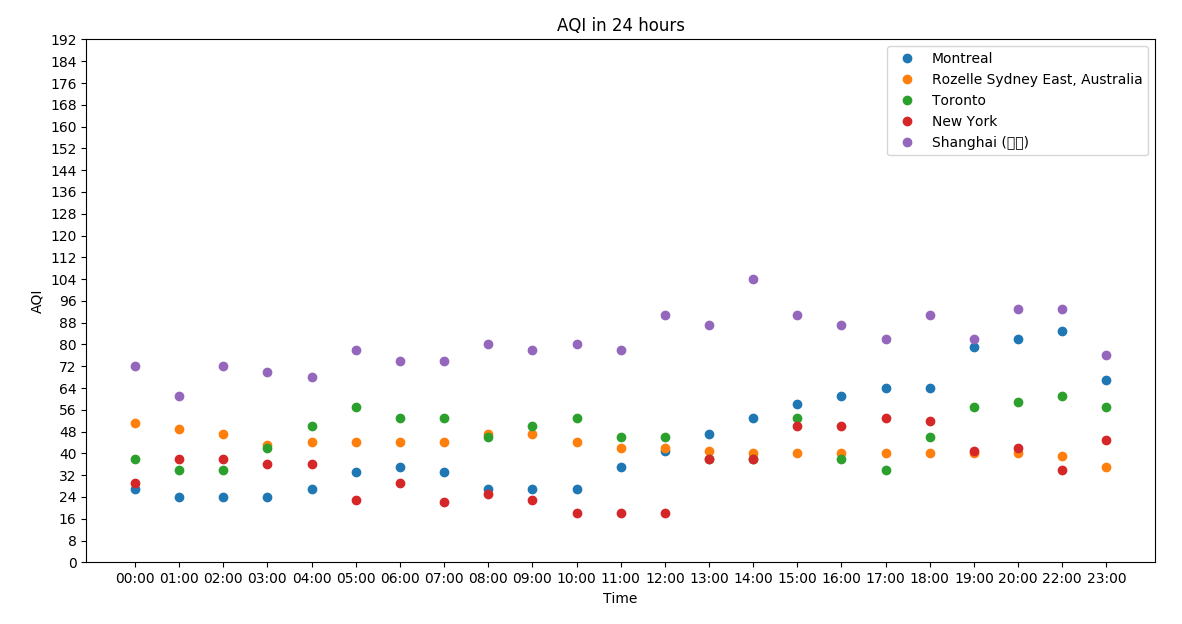
\includegraphics[scale=0.4]{aqi-graph-1}
	\caption{Air Quality Index Graph 1}
\end{figure}

\begin{figure}[h]
	\centering
	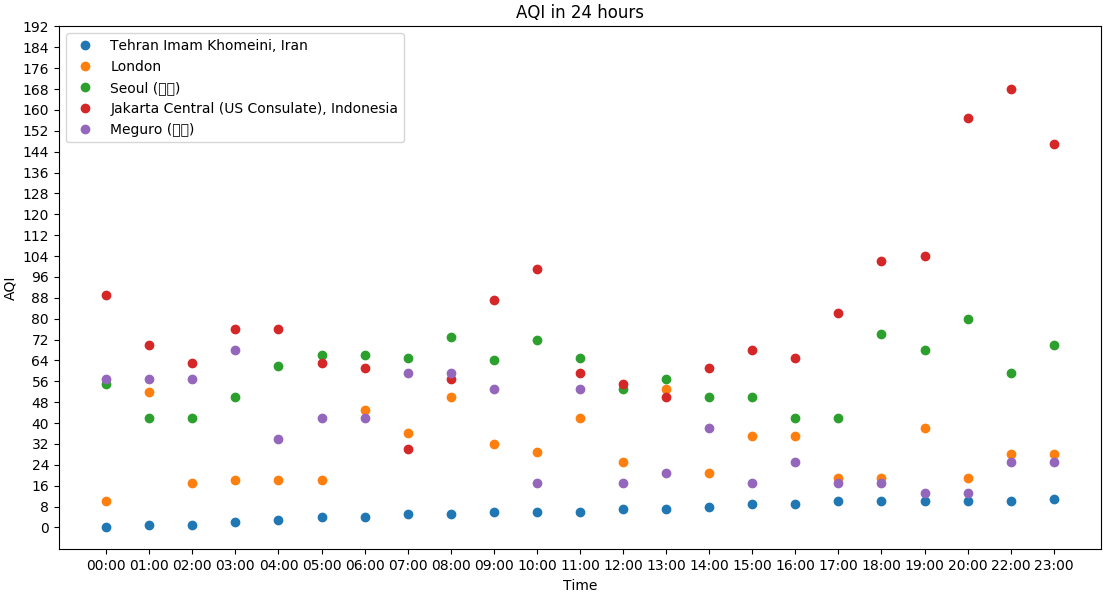
\includegraphics[scale=0.4]{aqi-graph-2}
	\caption{Air Quality Index Graph 2}
\end{figure}

\begin{figure}[h]
	\centering
	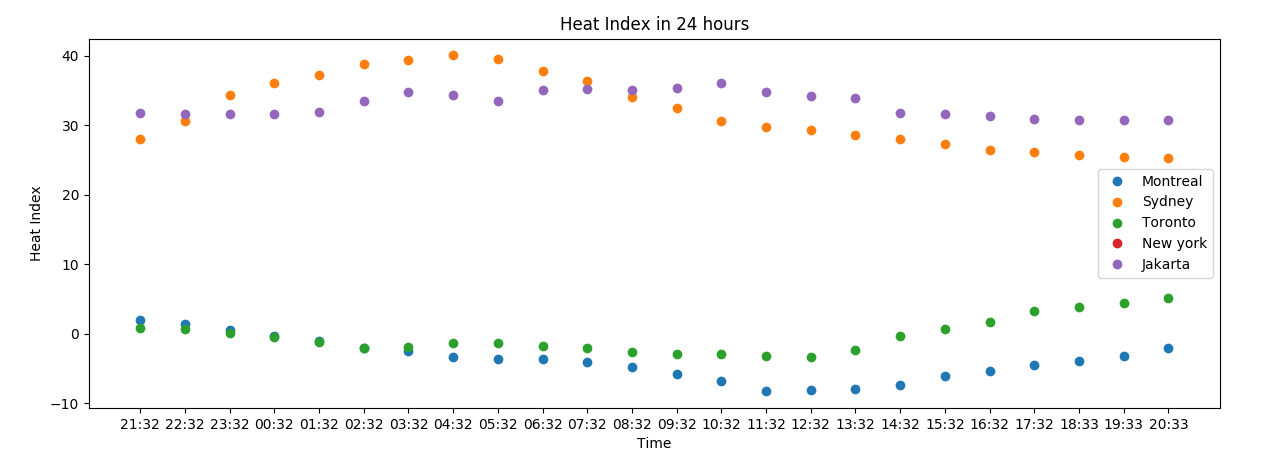
\includegraphics[scale=0.4]{hi-graph-1}
	\caption{Heat Index Graph 1}
\end{figure}

\begin{figure}[h]
	\centering
	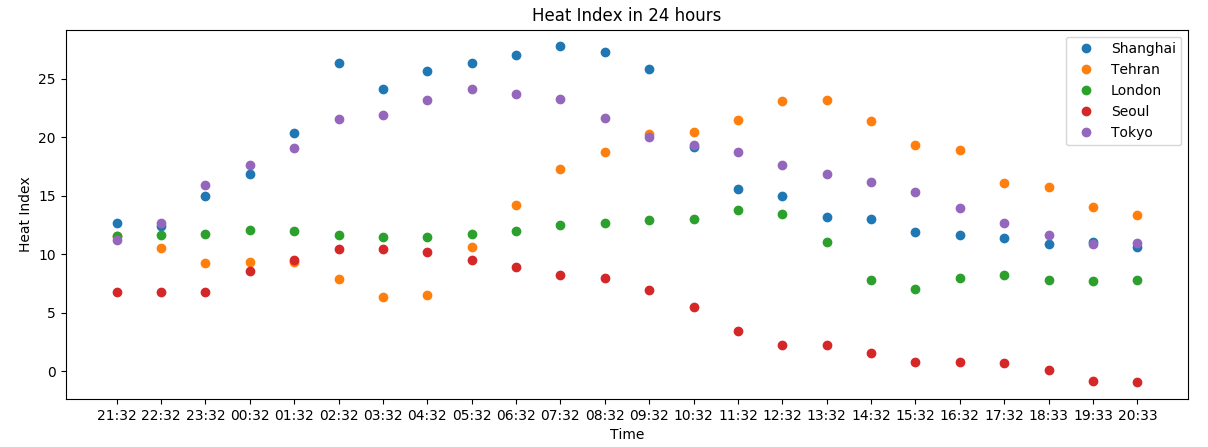
\includegraphics[scale=0.4]{hi-graph-2}
	\caption{Heat Index Graph 2}
\end{figure}
\end{document}
